% !TEX program = pdflatex
% FRE6883 Recitation 1 -- Financial problem, code, and hedge
\documentclass[10pt,aspectratio=169]{beamer}

% Language & encoding
\usepackage[utf8]{inputenc}
\usepackage[T1]{fontenc}
\usepackage[english]{babel}
\usepackage{lmodern}
\usepackage{microtype}

% Math / tables / layout
\usepackage{amsmath,amssymb,bm,mathtools}
\usepackage{booktabs}
\usepackage{multicol}
\usepackage{changepage}

% Graphics
\usepackage{graphicx}
\usepackage{tikz}
\usetikzlibrary{arrows.meta,positioning,calc,decorations.pathreplacing}
\usepackage{pgfplots}
\pgfplotsset{compat=1.18}

% Theme (Metropolis)
\usetheme[numbering=fraction,progressbar=frametitle]{metropolis}
\setbeamertemplate{frame numbering}[fraction]
\setbeamertemplate{navigation symbols}{}

% Bootcamp palette
\definecolor{BootcampBlueDark}{HTML}{1A3C68}
\definecolor{BootcampBlue}{RGB}{31,110,178}
\definecolor{AccentGold}{HTML}{DAA520}
\definecolor{SoftGray}{RGB}{245,246,248}
\definecolor{TextBlack}{HTML}{000000}
\definecolor{Crimson}{HTML}{990000}
\definecolor{MatrixGreen}{HTML}{228B22}
\definecolor{MatrixRed}{HTML}{B22222}

% Global formatting
\setbeamercolor{normal text}{fg=TextBlack,bg=white}
\setbeamercolor{title}{fg=TextBlack}
\setbeamercolor{structure}{fg=BootcampBlueDark}
\setbeamercolor{progress bar}{fg=BootcampBlueDark,bg=gray!30}

\setbeamercolor{frametitle}{bg=BootcampBlueDark,fg=white}
\setbeamerfont{frametitle}{series=\bfseries,size=\large}
\setbeamertemplate{frametitle}{
  \nointerlineskip
  \begin{beamercolorbox}[wd=\paperwidth,ht=3.2ex,dp=1.4ex,leftskip=1em,rightskip=1em]{frametitle}
    \usebeamerfont{frametitle}\insertframetitle
  \end{beamercolorbox}
}

\setbeamercolor{block title example}{bg=BootcampBlueDark!90!black,fg=white}
\setbeamercolor{block body example}{bg=BootcampBlueDark!5!white,fg=black}
\setbeamercolor{block title proposition}{bg=MatrixGreen!75!black,fg=white}
\setbeamercolor{block body proposition}{bg=MatrixGreen!7!white,fg=black}
\setbeamercolor{block title illustration}{bg=AccentGold!85!black,fg=white}
\setbeamercolor{block body illustration}{bg=AccentGold!10!white,fg=black}
\setbeamercolor{block title proof}{bg=gray!70!black,fg=white}
\setbeamercolor{block body proof}{bg=SoftGray,fg=black}
\setbeamertemplate{blocks}[rounded][shadow=false]

\newenvironment{definitionblock}[1]{%
  \par\vspace{0.4em}%
  \begin{beamercolorbox}[
      wd=\textwidth,sep=0.4em,leftskip=0.3em,rightskip=0.6em,
      rounded=false,shadow=false
    ]{block title example}%
    \raisebox{0.15em}{\usebeamerfont{block title example}#1}%
  \end{beamercolorbox}%
  \vspace{-0.4em}%
  \begin{beamercolorbox}[
      wd=\textwidth,sep=0.9em,leftskip=0.6em,rightskip=0.6em,
      rounded=false,shadow=false
    ]{block body example}%
    \usebeamerfont{block body example}%
}{%
  \end{beamercolorbox}%
  \par\vspace{0.6em}%
}

\newenvironment{propositionblock}[1]{%
  \par\vspace{0.35em}%
  \begin{beamercolorbox}[
      wd=\textwidth,sep=0.4em,leftskip=0.3em,rightskip=0.6em,
      rounded=false,shadow=false
    ]{block title proposition}%
    \raisebox{0.15em}{\usebeamerfont{block title example}#1}%
  \end{beamercolorbox}%
  \vspace{-0.4em}%
  \begin{beamercolorbox}[
      wd=\textwidth,sep=0.8em,leftskip=0.6em,rightskip=0.6em,
      rounded=false,shadow=false
    ]{block body proposition}%
    \usebeamerfont{block body example}%
}{%
  \end{beamercolorbox}%
  \par\vspace{0.55em}%
}

\newenvironment{illustrationblock}[1]{%
  \par\vspace{0.35em}%
  \begin{beamercolorbox}[
      wd=\textwidth,sep=0.4em,leftskip=0.3em,rightskip=0.6em,
      rounded=false,shadow=false
    ]{block title illustration}%
    \raisebox{0.15em}{\usebeamerfont{block title example}#1}%
  \end{beamercolorbox}%
  \vspace{-0.4em}%
  \begin{beamercolorbox}[
      wd=\textwidth,sep=0.8em,leftskip=0.6em,rightskip=0.6em,
      rounded=false,shadow=false
    ]{block body illustration}%
    \usebeamerfont{block body example}%
}{%
  \end{beamercolorbox}%
  \par\vspace{0.55em}%
}

\newenvironment{proofblock}[1]{%
  \par\vspace{0.3em}%
  \begin{beamercolorbox}[
      wd=\textwidth,sep=0.35em,leftskip=0.3em,rightskip=0.6em,
      rounded=false,shadow=false
    ]{block title proof}%
    \raisebox{0.15em}{\usebeamerfont{block title example}#1}%
  \end{beamercolorbox}%
  \vspace{-0.4em}%
  \begin{beamercolorbox}[
      wd=\textwidth,sep=0.7em,leftskip=0.6em,rightskip=0.6em,
      rounded=false,shadow=false
    ]{block body proof}%
    \usebeamerfont{block body example}%
}{%
  \end{beamercolorbox}%
  \par\vspace{0.45em}%
}


% Self-contained Deck 1. Theme, palette, and teaching-block macros above
% are inherited verbatim from the Fall 2026 FRE6233 Lecture 1 source.
% C++ listings follow the FRE6883 lecture conventions: explicit types,
% std:: qualification, braces on separate lines, and short // comments.
\usepackage{listings}
\lstdefinestyle{coursecpp}{
  language=C++,
  basicstyle=\ttfamily\fontsize{10}{11.5}\selectfont,
  keywordstyle=\color{blue},
  commentstyle=\color{MatrixGreen},
  stringstyle=\color{Crimson},
  showstringspaces=false,
  columns=fullflexible,
  keepspaces=true,
  tabsize=4,
  breaklines=false,
  frame=none,
  aboveskip=0.5em,
  belowskip=0.5em
}
\lstset{style=coursecpp}
\setbeamercovered{invisible}


\title{From a Financial Problem to C++ Code}
\author{}
\date{}
% This file is self-contained: no external figures, code, or theme files beyond
% standard TeX packages. Compile with pdfLaTeX twice or latexmk -pdf.
% Sources: FRE6883 Topic 2 updated, pp. 7-12, 14-25, 28-37.
% Theme and macros: Fall 2026 FRE6233 Lecture 1, inherited through Deck 0.
% User-requested scope supersedes the original six-frame, 25-minute outline.
% Financial assumptions: non-dividend-paying stock, European call, frictionless
% binomial model, constant positive gross factors 0 < D < R < U, S0 > 0.
% One-step example: S0=100, U=1.2, D=.8, R=1.1, K=100.
% N=2 means two steps with the same per-step factors, not a rescaled horizon.
% Technical accuracy: use R <= D, correcting Topic 2 pp. 24-25's repeated U <= D.
% Price uses fixed compile-time capacity SIZE=9 and a guard for 1<=N<=8.
% The adapted pricer keeps the lecture's function signature, namespace, helper
% names, loop directions, in-place Price row, and return value. It only adds
% two stock-node calculations and delta output before the original update.
% Presenter guidance: let students attempt each question before revealing.
% If Deck 0 showed weak syntax fluency, accept pseudocode and trace values aloud.
% Functions and arrays are introduced locally; detailed syntax practice follows.
% Do not turn the probability formula into a pricing-theory derivation.
% Substantial exercises have separate solution frames; timings include work.
\begin{document}
% FRAME 1: 0.5 minutes. Welcome; no Topic 2 completion is assumed.
\begin{frame}[plain]
\vfill
{\usebeamerfont{title}\inserttitle\par}
\medskip
{\color{BootcampBlueDark}\rule{0.95\textwidth}{0.8pt}}
\bigskip
{\Large FRE6883 -- Recitation 1\par}
\medskip
One period, a tree, and a replicating hedge
\vfill
\end{frame}

% FRAME 2: 2.0 minutes. 
\begin{frame}{One period: two possible stock prices}
\relax

\begin{columns}[c,onlytextwidth]
\begin{column}{0.49\textwidth}
\centering
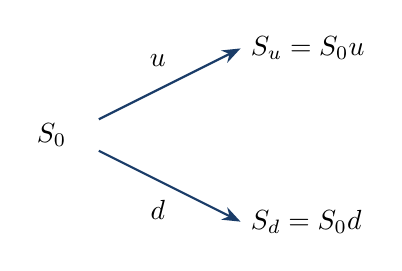
\begin{tikzpicture}[>=Stealth,thick]
\draw[->,BootcampBlueDark] (0.6,0.2) -- (2.4,1.1);
\draw[->,BootcampBlueDark] (0.6,-0.2) -- (2.4,-1.1);
\node at (0,0) {$S_0$};
\node[right] at (2.4,1.1) {$S_u=S_0u$};
\node[right] at (2.4,-1.1) {$S_d=S_0d$};
\node at (1.35,0.95) {$u$};
\node at (1.35,-0.95) {$d$};
\end{tikzpicture}
\end{column}
\begin{column}{0.48\textwidth}
\begin{definitionblock}{A European call at expiry}
$H_u=\max(S_u-K,0)$\par\medskip
$H_d=\max(S_d-K,0)$
\end{definitionblock}
\end{column}
\end{columns}
\medskip
\textbf{Example:} $S_0=100$, $u=1.2$, $d=0.8$, $R=1.1$, $K=100$.\par
{\small $R$ is a gross growth factor: one risk-free dollar becomes $R$ dollars.}
\smallskip\par
\textbf{Predict:} in which state does the call pay something?

\end{frame}

% FRAME 3: 2.0 minutes. Let pairs propose the order before the second overlay; no probability derivation.
\begin{frame}{Explain the procedure to a computer}
\relax

\begin{definitionblock}{Pricing rule}
\[
q=\frac{R-d}{u-d},\qquad H_0=\frac{qH_u+(1-q)H_d}{R}.
\]
$q$ supplies the pricing weights; divide by $R$ to express the result today.
\end{definitionblock}
\begin{overlayarea}{\textwidth}{2.2cm}
\only<1>{\medskip Write the steps in plain English before writing any C++.\par
\smallskip Assume $S_0>0$, $K\geq0$, and $0<d<R<u$.}
\only<2>{\small
Define/read and check parameters $\to$ compute $S_u,S_d$ $\to$ compute $H_u,H_d$\par\medskip
Compute $q$ $\to$ compute $H_0$ $\to$ display the result.\par\medskip
The pricing weights sum to one; $q$ is not a forecast of the up-state frequency.}
\end{overlayarea}

\end{frame}

% FRAME 4: 1.5 minutes. 
\begin{frame}{Which variables and types do we need?}
\relax

\textbf{Choose a C++ type for prices, growth factors, and a step count.}
\begin{overlayarea}{\textwidth}{4.0cm}
\only<1>{\begin{illustrationblock}{Start with the inputs}
$S_0=100$, $u=1.2$, $d=0.8$, $R=1.1$, $K=100$.\par\medskip
Would an integer type preserve every input?
\end{illustrationblock}}
\only<2>{
\begin{definitionblock}{Course notation in main()}
\texttt{double s0 = 100.0, k = 100.0;}\par\medskip
\texttt{double u = 1.2, d = 0.8, r = 1.1;}
\end{definitionblock}
Use \texttt{double} for the computed prices and probabilities too.\par
Use \texttt{int} for step counts and node indices.}
\end{overlayarea}
{\small Course convention: lower-case inputs in \texttt{main()}; $S0,U,D,R$ in model functions.}

\end{frame}

% FRAME 5: 1.0 minutes. 
\begin{frame}[fragile]{Compute the two stock prices}
\relax

\textbf{Complete the right-hand sides before the reveal.}
\begin{lstlisting}
double Su = /* ? */;
double Sd = /* ? */;
\end{lstlisting}
\begin{overlayarea}{\textwidth}{2.8cm}
\only<2>{\begin{propositionblock}{Multiply the initial price by each factor}
\texttt{double Su = s0 * u;}\qquad $S_u=120$\par\medskip
\texttt{double Sd = s0 * d;}\qquad $S_d=80$
\end{propositionblock}}
\end{overlayarea}
{\small Code fragments in this part belong inside \texttt{int main()}.}

\end{frame}

% FRAME 6: 1.5 minutes. 
\begin{frame}[fragile]{Implement the positive part}
\relax

\textbf{How can the program ensure that a call payoff is never negative?}
\begin{columns}[T,onlytextwidth]
\begin{column}{0.50\textwidth}
\begin{lstlisting}
double Hu = 0.0;
if (Su > k)
{
    Hu = Su - k;
}
\end{lstlisting}
\end{column}
\begin{column}{0.46\textwidth}
\begin{overlayarea}{\linewidth}{3.4cm}
\only<1>{\begin{illustrationblock}{Predict}
What is \texttt{Hu} when $S_u=K$?\par\medskip
Would an \texttt{else} branch change the answer?
\end{illustrationblock}}
\only<2>{\begin{propositionblock}{At the strike, the payoff is zero}
Initialization already covers the other case. An explicit \texttt{else} could assign \texttt{0.0} again.
\end{propositionblock}}
\end{overlayarea}
\end{column}
\end{columns}
{\small Alternative: \texttt{std::max(Su - k, 0.0)} needs \texttt{<algorithm>}.\par
We keep the professor's conditional-payoff style; repeat it for \texttt{Hd}.}

\end{frame}

% FRAME 7: 2.0 minutes. 
\begin{frame}[fragile]{Compute the price and display it}
\relax

\textbf{Which parentheses belong in the two missing expressions?}
\begin{lstlisting}
double q = /* (r - d) divided by (u - d) */;
double optionPrice = /* weighted payoff divided by r */;
\end{lstlisting}
\begin{overlayarea}{\textwidth}{3.3cm}
\only<2>{
\begin{propositionblock}{Translate the formulas directly}
\texttt{double q = (r - d) / (u - d);}\par\medskip
\texttt{double optionPrice = (q * Hu + (1.0 - q) * Hd) / r;}
\end{propositionblock}
$q=0.75$ and $H_0=15/1.1\approx13.6364$.}
\end{overlayarea}
% Output uses <iostream> and <iomanip>, shown in the complete solution.
\begin{lstlisting}[basicstyle=\ttfamily\fontsize{8.5}{10}\selectfont]
std::cout << std::fixed << std::setprecision(2)
          << optionPrice << std::endl;
\end{lstlisting}

\end{frame}

% FRAME 8: 4.0 minutes. At least 2.5 minutes individual/pair work. Do not advance to the solution early.
\begin{frame}[fragile]{Exercise: complete the one-period pricer}
\relax

{\small Inside \texttt{main()}; headers and numeric inputs are supplied. Fill all blanks, then predict the printed result.}
\begin{lstlisting}[basicstyle=\ttfamily\fontsize{8.5}{9}\selectfont]
double s0 = 100.0, k = 100.0;
double u = 1.2, d = 0.8, r = 1.1;
double Su = /* A */, Sd = /* B */;
double Hu = 0.0, Hd = 0.0;
if (/* C */)
{
    Hu = /* D */;
}
if (/* E */)
{
    Hd = /* F */;
}
double q = /* G */;
double optionPrice = /* H */;
std::cout << std::fixed << std::setprecision(2)
          << optionPrice << std::endl;
\end{lstlisting}

\end{frame}

% FRAME 9: 2.0 minutes. 
\begin{frame}[fragile]{Solution: a complete one-period program}
\relax

{\small Read the left column, then continue on the right. Inputs satisfy $S_0>0$, $K\geq0$, $0<d<R<u$.}
\begin{columns}[T,onlytextwidth]
\begin{column}{0.49\textwidth}
\begin{lstlisting}[basicstyle=\ttfamily\fontsize{8.5}{10}\selectfont]
#include <iostream>
#include <iomanip>
int main()
{
    double s0 = 100.0, k = 100.0;
    double u = 1.2, d = 0.8, r = 1.1;
    double Su = s0 * u, Sd = s0 * d;
    double Hu = 0.0, Hd = 0.0;
    if (Su > k)
    {
        Hu = Su - k;
    }
\end{lstlisting}
\end{column}
\begin{column}{0.48\textwidth}
\begin{lstlisting}[basicstyle=\ttfamily\fontsize{8.5}{10}\selectfont]
    if (Sd > k)
    {
        Hd = Sd - k;
    }
    double q = (r - d) / (u - d);
    double optionPrice =
        (q * Hu + (1.0 - q) * Hd) / r;
    std::cout << std::fixed
              << std::setprecision(2)
              << optionPrice << std::endl;
    return 0;
}
\end{lstlisting}
\end{column}
\end{columns}
\textbf{Output:} \texttt{13.64}.\quad \textbf{Check:} if $K=120$, both payoffs and the price are zero.

\end{frame}

% FRAME 10: 1.0 minutes. 
\begin{frame}{How do we avoid writing every node manually?}
\relax

\begin{center}
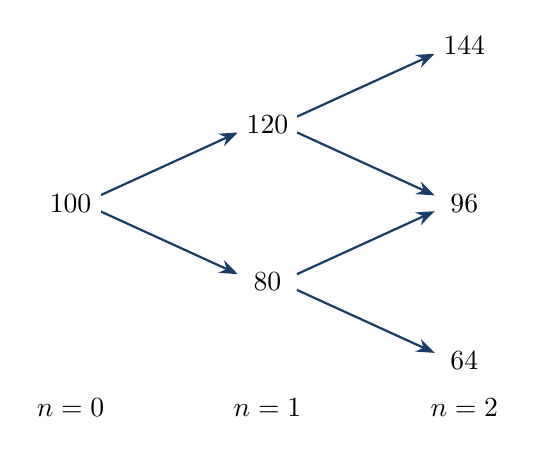
\begin{tikzpicture}[>=Stealth,thick,x=2.5cm,y=1.0cm]
\draw[->,BootcampBlueDark] (0.15,0.1)--(0.85,0.9);
\draw[->,BootcampBlueDark] (0.15,-0.1)--(0.85,-0.9);
\draw[->,BootcampBlueDark] (1.15,1.1)--(1.85,1.9);
\draw[->,BootcampBlueDark] (1.15,0.9)--(1.85,0.1);
\draw[->,BootcampBlueDark] (1.15,-0.9)--(1.85,-0.1);
\draw[->,BootcampBlueDark] (1.15,-1.1)--(1.85,-1.9);
\node[fill=white] at (0,0) {100};
\node[fill=white] at (1,1) {120}; \node[fill=white] at (1,-1) {80};
\node[fill=white] at (2,2) {144}; \node[fill=white] at (2,0) {96};
\node[fill=white] at (2,-2) {64};
\node at (0,-2.6) {$n=0$}; \node at (1,-2.6) {$n=1$}; \node at (2,-2.6) {$n=2$};
\end{tikzpicture}
\end{center}
\textbf{Predict:} how many distinct stock-price nodes are there at time 2?

\end{frame}

% FRAME 11: 1.5 minutes. 
\begin{frame}[fragile]{One formula describes every stock-price node}
\relax

\[
\boxed{S(n,i)=S_0u^i d^{\,n-i}},\qquad 0\leq i\leq n.
\]
$n$: number of elapsed steps.\quad $i$: number of up moves.\par\medskip
There are $n-i$ down moves and $n+1$ distinct nodes at time $n$.
\begin{lstlisting}
s0 * std::pow(u, i) * std::pow(d, n - i)
\end{lstlisting}
{\small \texttt{std::pow} comes from \texttt{<cmath>}; \texttt{n} and \texttt{i} are integers.}
\begin{overlayarea}{\textwidth}{2.2cm}
\only<1>{\begin{illustrationblock}{Quick check}
What are $(n,i)$ and the stock price after one up move and one down move?
\end{illustrationblock}}
\only<2>{\begin{propositionblock}{Two steps, one up move}
$(n,i)=(2,1)$, so $S(2,1)=100(1.2)(0.8)=96$.
\end{propositionblock}}
\end{overlayarea}

\end{frame}

% FRAME 12: 2.0 minutes. Keep the preceding formula visible verbally; teach for initialization/condition/update locally.
\begin{frame}[fragile]{Exercise: complete the nested loops}
\relax

\begin{lstlisting}
const int N = 2;
for (int n = 0; n <= N; n++)
{
    for (int i = /* ? */; /* ? */; /* ? */)
    {
        std::cout << n << " " << i << " "
                  << /* stock price */ << std::endl;
    }
}
\end{lstlisting}
\textbf{Explain your bounds:}
\begin{itemize}
\item What do \texttt{n} and \texttt{i} represent? Why must \texttt{i <= n}?
\item How many nodes are printed at time \texttt{n}? How many in total for $N=2$?
\end{itemize}

\end{frame}

% FRAME 13: 1.0 minutes. 
\begin{frame}[fragile]{Solution: visit each node once}
\relax

\begin{lstlisting}[basicstyle=\ttfamily\fontsize{8.5}{10}\selectfont]
const int N = 2;
for (int n = 0; n <= N; n++)
{
    for (int i = 0; i <= n; i++)
    {
        std::cout << n << " " << i << " "
                  << s0 * std::pow(u, i)
                        * std::pow(d, n - i) << std::endl;
    }
}
\end{lstlisting}
\begin{propositionblock}{Check the traversal}
$n$ selects the time level; $i=0,\ldots,n$ visits its $n+1$ nodes.\par
For $N=2$: $1+2+3=6$ nodes. At $n=2$, prices print as $64,96,144$.
\end{propositionblock}

\end{frame}

% FRAME 14: 1.5 minutes. 
\begin{frame}[fragile]{When will we need to keep a computed value?}
\relax

Printing a stock price is enough to inspect it. Pricing backward requires the next level's option values again.
\begin{lstlisting}
const int SIZE = 9;
double Price[SIZE] = { 0.0 };
\end{lstlisting}
\begin{definitionblock}{An array is an indexed row of values}
\texttt{Price[0]}, \texttt{Price[1]}, \ldots, \texttt{Price[8]} are nine \texttt{double} slots.\par
The valid indices are $0$ through $8$; the array does not check the bounds for us.
\end{definitionblock}
\textbf{For $N=2$:} terminal call payoffs are $[0,0,44]$.\par
\textbf{Ask:} do we need to store the entire tree to reuse one level?\par
{\small We will keep one level in \texttt{Price}; Deck 2 will revisit array syntax.}

\end{frame}

% FRAME 15: 2.0 minutes. 
\begin{frame}{A hedge must match both option payoffs}
\relax

\begin{definitionblock}{Replicate one long call}
Hold $\Delta$ shares and invest $B$ dollars in the risk-free asset today.\par
At the next step, the cash position is worth $BR$.
\end{definitionblock}
\[
\begin{aligned}
\Delta S_u+BR&=H_u,\\[0.4em]
\Delta S_d+BR&=H_d.
\end{aligned}
\]
\textbf{Ask:} what disappears if we subtract the second equation from the first?\par\medskip
$B<0$ means borrowing. The initial cost is $\Delta S_0+B$.

\end{frame}

% FRAME 16: 1.5 minutes. 
\begin{frame}{Delta is the number of shares in the hedge}
\relax

\[
\Delta(S_u-S_d)=H_u-H_d
\quad\Longrightarrow\quad
\boxed{\Delta=\frac{H_u-H_d}{S_u-S_d}}.
\]
\begin{propositionblock}{Interpret the ratio}
The option's change between states, divided by the stock's change, gives the number of shares needed to replicate one option.
\end{propositionblock}
Then compute the cash position and the cost:
\[
B=\frac{H_d-\Delta S_d}{R},\qquad H_0=\Delta S_0+B.
\]
\textbf{Predict:} if both call payoffs are zero, what is $\Delta$?\par
{\small To hedge a short call, hold this replicating portfolio.}

\end{frame}

% FRAME 17: 3.0 minutes. Allow two minutes work before discussion. Finance is a supplied computational recipe.
\begin{frame}{Exercise: compute and interpret the hedge}
\relax

\textbf{Use the same inputs:} $S_0=100$, $u=1.2$, $d=0.8$, $R=1.1$, $K=100$.
\begin{columns}[T,onlytextwidth]
\begin{column}{0.48\textwidth}
\begin{enumerate}\setlength{\itemsep}{0.5em}
\item Compute $S_u$ and $S_d$.
\item Compute $H_u$ and $H_d$.
\item Compute $q$ and $H_0$.
\item Compute $\Delta$.
\item Explain what $\Delta$ means.
\end{enumerate}
\end{column}
\begin{column}{0.48\textwidth}
\begin{definitionblock}{Useful formulas}
$q=(R-d)/(u-d)$\par\medskip
$H_0=(qH_u+(1-q)H_d)/R$\par\medskip
$\Delta=(H_u-H_d)/(S_u-S_d)$
\end{definitionblock}
\end{column}
\end{columns}
\medskip
\textbf{If finished:} find $B$ and check the portfolio in both states.

\end{frame}

% FRAME 18: 2.0 minutes. 
\begin{frame}{Solution: half a share and a cash position}
\relax

\begin{columns}[T,onlytextwidth]
\begin{column}{0.48\textwidth}
\begin{propositionblock}{Price and delta}
$S_u=120$, $S_d=80$\par\medskip
$H_u=20$, $H_d=0$, $q=0.75$\par\medskip
$H_0=15/1.1\approx13.6364$\par\medskip
$\Delta=(20-0)/(120-80)=0.5$
\end{propositionblock}
\end{column}
\begin{column}{0.48\textwidth}
\begin{definitionblock}{Check replication}
$B=(0-0.5\cdot80)/1.1$\par
$B\approx-36.3636$, so $BR=-40$.\par\medskip
Up: $0.5\cdot120-40=20$.\par
Down: $0.5\cdot80-40=0$.\par\medskip
Cost: $0.5\cdot100+B\approx13.6364$.
\end{definitionblock}
\end{column}
\end{columns}
\medskip
\textbf{Interpretation:} hold half a share per call and borrow about 36.36 today.\par
{\small Compute with full precision; round only the displayed result.}

\end{frame}

% FRAME 19: 1.5 minutes. These terms are introduced here; no prior reference knowledge is required. Vote before revealing next slide.
\begin{frame}{Design a function that computes delta}
\relax

\textbf{Before seeing the function, decide:}
\begin{enumerate}\setlength{\itemsep}{0.4em}
\item What is the return type?
\item Which four arguments are needed?
\item Does the function need to modify any of them?
\item Should these parameters be passed by value or reference?
\item Which expression should be returned?
\end{enumerate}
\begin{definitionblock}{Just enough function vocabulary}
Arguments supply inputs; \texttt{return} sends back the result.\par
By value gives the function a copy. A reference names the caller's variable.
\end{definitionblock}
{\small Use the name \texttt{CalculateDelta}, consistent with \texttt{CalculateAssetPrice}.}

\end{frame}

% FRAME 20: 1.0 minutes. 
\begin{frame}[fragile]{Solution: return one double from four inputs}
\relax

\begin{lstlisting}
namespace fre {
    double CalculateDelta(double Su, double Sd,
                          double Hu, double Hd)
    {
        return (Hu - Hd) / (Su - Sd);
    }
}
\end{lstlisting}
\begin{lstlisting}
double delta = fre::CalculateDelta(Su, Sd, Hu, Hd);
\end{lstlisting}
\textbf{By value is sufficient:} these four numeric inputs do not need to change.\par
{\small \texttt{fre::} selects the function in the course namespace. Define it before \texttt{main()} for a one-file program. Assume $S_u>S_d$ before dividing.}

\end{frame}

% FRAME 21: 1.5 minutes. 
\begin{frame}{The same hedge works locally in a CRR tree}
\relax

\begin{center}
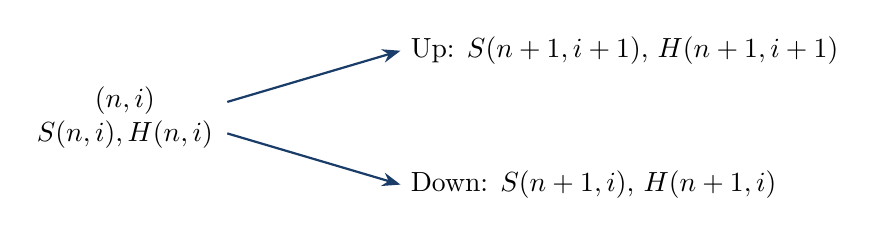
\begin{tikzpicture}[>=Stealth,thick]
\draw[->,BootcampBlueDark] (1.3,0.2)--(3.5,0.85);
\draw[->,BootcampBlueDark] (1.3,-0.2)--(3.5,-0.85);
\node[align=center] at (0,0) {$(n,i)$\\$S(n,i),H(n,i)$};
\node[right,align=left] at (3.5,0.85) {Up: $S(n+1,i+1)$, $H(n+1,i+1)$};
\node[right,align=left] at (3.5,-0.85) {Down: $S(n+1,i)$, $H(n+1,i)$};
\end{tikzpicture}
\end{center}
\[
\boxed{\Delta(n,i)=\frac{H(n+1,i+1)-H(n+1,i)}
{S(n+1,i+1)-S(n+1,i)}}
\]
Once the two next-period option values are known, we can compute the current hedge. Recompute it at each visited non-terminal node.\par\smallskip
\textbf{Ask:} are these option values always terminal payoffs?\par
{\small Only on the last step; earlier they are continuation values found by pricing backward.}

\end{frame}

% FRAME 22: 1.5 minutes. 
\begin{frame}[fragile]{Read one backward-induction update}
\relax

At time $n$, the active array entries still hold time-$n+1$ option values:
\[
\texttt{Price[i]}=H(n+1,i),\qquad
\texttt{Price[i+1]}=H(n+1,i+1).
\]
\begin{lstlisting}
Price[i] = (q * Price[i + 1]
         + (1.0 - q) * Price[i]) / R;
\end{lstlisting}
After this line, \texttt{Price[i]} holds $H(n,i)$ instead.\par\medskip
\textbf{Predict:} for our two-step example, terminal values $[0,0,44]$ become what at time 1?
\begin{overlayarea}{\textwidth}{2.2cm}
\only<2>{\begin{propositionblock}{The active row becomes $[0,30]$}
$H(1,0)=0$, and $H(1,1)=(0.75\cdot44)/1.1=30$.
\end{propositionblock}}
\end{overlayarea}

\end{frame}

% FRAME 23: 3.0 minutes. Allow two minutes work. Ask students to mark which entries still belong to n+1.
\begin{frame}[fragile]{Exercise: compute the hedge before losing data}
\relax

\begin{lstlisting}[basicstyle=\ttfamily\fontsize{8.5}{10}\selectfont]
for (int n = N - 1; n >= 0; n--)
{
    for (int i = 0; i <= n; i++)
    {
        // A: compute the two next-period stock prices
        // B: compute and display delta
        // C: replace Price[i] by the current option price
    }
}
\end{lstlisting}
\textbf{Complete the algorithm in words or C++:}
\begin{itemize}
\item Which option entries and stock nodes belong in the delta formula?
\item Why must B come before C? Why visit \texttt{i} from left to right?
\end{itemize}
\textbf{Trace at the root:} old row $[0,30]$, stock children $[80,120]$.\par
What goes wrong if \texttt{Price[0]} is replaced first?

\end{frame}

% FRAME 24: 2.0 minutes. 
\begin{frame}{Solution: use both children, then overwrite}
\relax

\begin{enumerate}\setlength{\itemsep}{0.3em}
\item Compute $S_u=S(n+1,i+1)$ and $S_d=S(n+1,i)$.
\item Compute $\Delta=(\texttt{Price[i+1]}-\texttt{Price[i]})/(S_u-S_d)$.
\item Display delta, then apply the usual pricing update to \texttt{Price[i]}.
\end{enumerate}
\begin{columns}[T,onlytextwidth]
\begin{column}{0.48\textwidth}
\begin{propositionblock}{Correct root calculation}
Old option row: $[0,30]$.\par
$\Delta(0,0)=(30-0)/(120-80)=0.75$.\par
Then $H(0,0)=0.75\cdot30/1.1\approx20.4545$.
\end{propositionblock}
\end{column}
\begin{column}{0.48\textwidth}
\begin{illustrationblock}{If you overwrite first}
$(30-20.4545)/(120-80)\approx0.2386$.\par\smallskip
This mixes values from two different time levels.
\end{illustrationblock}
\end{column}
\end{columns}
{\small Increasing \texttt{i} preserves both needed children until use; decreasing \texttt{i} would overwrite the next child's value too early.}

\end{frame}

% FRAME 25: 1.0 minutes. Read the purpose of the guard and initialization; array mechanics will be revisited in Deck 2.
\begin{frame}[fragile]{Prepare the terminal row in the existing pricer}
\relax

{\small Within \texttt{fre::PriceByCRR(S0, U, D, R, N, K)}: check inputs, then initialize.}
\begin{columns}[T,onlytextwidth]
\begin{column}{0.48\textwidth}
\begin{lstlisting}[basicstyle=\ttfamily\fontsize{8.5}{10}\selectfont]
const int SIZE = 9;
if (N < 1 || N >= SIZE
    || S0 <= 0.0 || K < 0.0
    || D <= 0.0 || U <= D
    || R <= D || R >= U)
{
    std::cerr << "Invalid model data"
              << std::endl;
    return -1.0;
}
\end{lstlisting}
\end{column}
\begin{column}{0.48\textwidth}
\begin{lstlisting}[basicstyle=\ttfamily\fontsize{8.5}{10}\selectfont]
double q = RiskNeutProb(U, D, R);
double Price[SIZE] = { 0.0 };
for (int i = 0; i <= N; i++)
{
    Price[i] = CallPayoff(
        CalculateAssetPrice(
            S0, U, D, N, i), K);
}
\end{lstlisting}
\end{column}
\end{columns}
\medskip
\texttt{SIZE = 9} supports $1\leq N\leq8$. The array holds one level.\par
{\small \texttt{CallPayoff} computes the positive part; \texttt{CalculateAssetPrice} implements the stock-node formula.}
% Course signature: double PriceByCRR(double S0, double U, double D,
%                                    double R, const int N, double K)
\end{frame}

% FRAME 26: 2.0 minutes. 
\begin{frame}[fragile]{Augment the existing CRR loop}
\relax

% Continue inside fre::PriceByCRR; CalculateDelta is also defined in fre.
\begin{lstlisting}[basicstyle=\ttfamily\fontsize{8.5}{10}\selectfont]
for (int n = N - 1; n >= 0; n--)
{
    for (int i = 0; i <= n; i++)
    {
        double Su = CalculateAssetPrice(S0, U, D, n + 1, i + 1);
        double Sd = CalculateAssetPrice(S0, U, D, n + 1, i);
        double delta = CalculateDelta(Su, Sd, Price[i + 1], Price[i]);
        std::cout << "Delta(" << n << "," << i << ") = "
                  << delta << std::endl;
        Price[i] = (q * Price[i + 1]
                 + (1.0 - q) * Price[i]) / R;
    }
}
return Price[0];
\end{lstlisting}
{\small $N=2$: $\Delta(1,0)=0$, $\Delta(1,1)\approx0.9167$, $\Delta(0,0)=0.75$; price $\approx20.4545$.}

\end{frame}

% FRAME 27: 1.0 minutes. 
\begin{frame}{From Finance to Code}
\relax

\begin{columns}[c,onlytextwidth]
\begin{column}{0.44\textwidth}
\centering
Financial model\par
$\downarrow$\par
Mathematical formulas\par
$\downarrow$\par
Algorithm\par
$\downarrow$\par
C++ implementation\par
$\downarrow$\par
Option price\par
$\downarrow$\par
Delta hedge
\end{column}
\begin{column}{0.52\textwidth}
\begin{propositionblock}{One tree, two computations}
The binomial tree gives both option values and the shares needed for the local replicating hedge.
\end{propositionblock}
\textbf{Exit question:} why must delta be computed before overwriting \texttt{Price[i]}?\par\medskip
Next: practise the C++ syntax that makes these steps work.
\end{column}
\end{columns}

\end{frame}

\end{document}
